\documentclass[a4paper, 12pt]{article}
\usepackage[english]{babel}
\usepackage[margin=1in]{geometry}
\usepackage{graphicx}
\usepackage{setspace}
\usepackage{multicol}
\usepackage{float}
\usepackage{subfig}
\usepackage{wrapfig}
\usepackage{hyperref}
\usepackage{booktabs}
\usepackage{gensymb}
\usepackage{csquotes}

\doublespacing

\graphicspath{{img}}

\setcounter{section}{-1}

\title{\Large EEE102 - 03 \qquad Lab Report 03\\ \small \hrulefill}
\date{}
\author{Selim Mert TOKER 22302352}

\begin{document}

\maketitle

\section{Introduction}

Aim of this lab is to practice assembling logic circuits on a breadboard, using multiple logic ICs, and retrieving information from a datasheet.


A logic circuit made up of two logic gate ICs (74HCxx) will be connected to process 4 input bits and output a single bit.
Four red LEDs are used to visualize the values of these bits (connected as stated in LEDcircuit.jpg).
In order to test the circuit for all possible combinations of the 4-bit input, a counter IC (74HC163) will be used, alongside with a signal generator for clock and an oscilloscope for monitoring the output.

\section{Assembling the Circuit}

\begin{wrapfigure}{r}{0.48\textwidth}
	\centering
	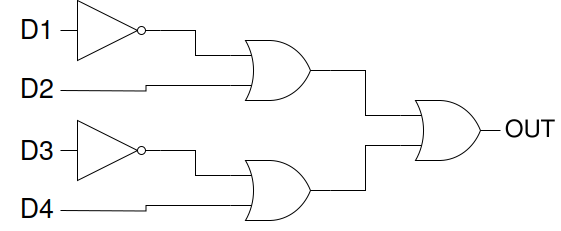
\includegraphics[width=0.48\textwidth]{diagram.png}
	\caption{Logic Gates}
	\label{fig:diagram}
\end{wrapfigure}

The two logic ICs are chosen to be 74HC04 (NOT gate) and 74HC32 (OR gate), attached to the breadboard and are connected to power according to their datasheet.
The two logic gate ICs are then connected to each other as shown in figure \ref{fig:diagram}.

Then, the counter IC 74HC163 is placed on the breadboard, and is connected to power and provided required signals (Count Enable and Clock Signal), .
The 4 output bits of the counter IC are connected to both the inputs of the logic circuit, and 4 LEDs (over 330$\Omega$ resistors to limit their current).
Finally, the output of the logic circuit is connected to an LED, over a 330$\Omega$ resistor, according to the schematic in \ref{fig:sch}, as seen on figure \ref{fig:circuit}.

The actual ICs, unlike the diagrams, have more pins that needs to be connected:
each IC has GND and Vcc pins for power.
Moreover, the counter IC (74HC163) has configuration pins, such as the MR (Master Reset, Pin 1), CEP (Counter Enable Input Pin 7), PE (Parallel Enable Input, Pin 9), CET (Count Enable Carry Input, Pin 10); which change the IC's mode, and has to be connected to either GND or +5V to set it up properly.
If the configuration pins are not connected to anywhere, they may pick up random parasite from environment and change the IC's mode in the midst of operation, messing the output up.

\begin{figure}
	\centering
	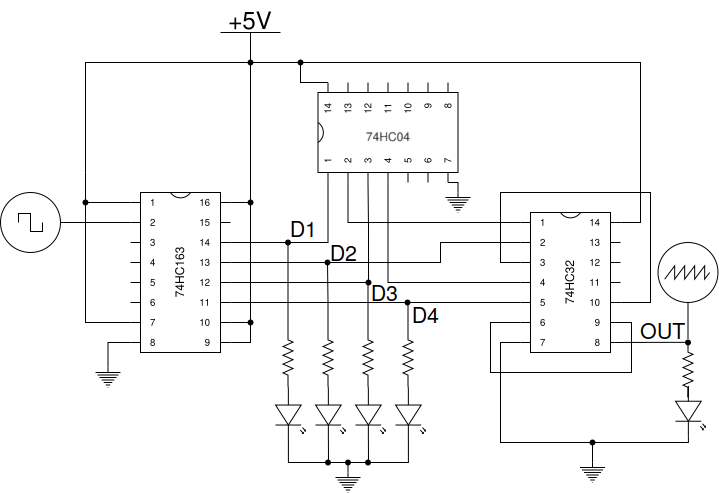
\includegraphics[width=\textwidth]{sch.png}
	\caption{Circuit Schematic}
	\label{fig:sch}
\end{figure}

With the clock signal set to 1Hz 5Vpp, and the oscilloscope connected to the output of the circuit, the board is connected to power and the LEDs are observed to be blinking, as expected.
The reason for such slow clock is to clearly see the LEDs turn on and off, as clock speeds greater than 20Hz cause the LEDs blink faster that a human eye can see.
\begin{figure}
	\vspace{-1cm}
	\centering
	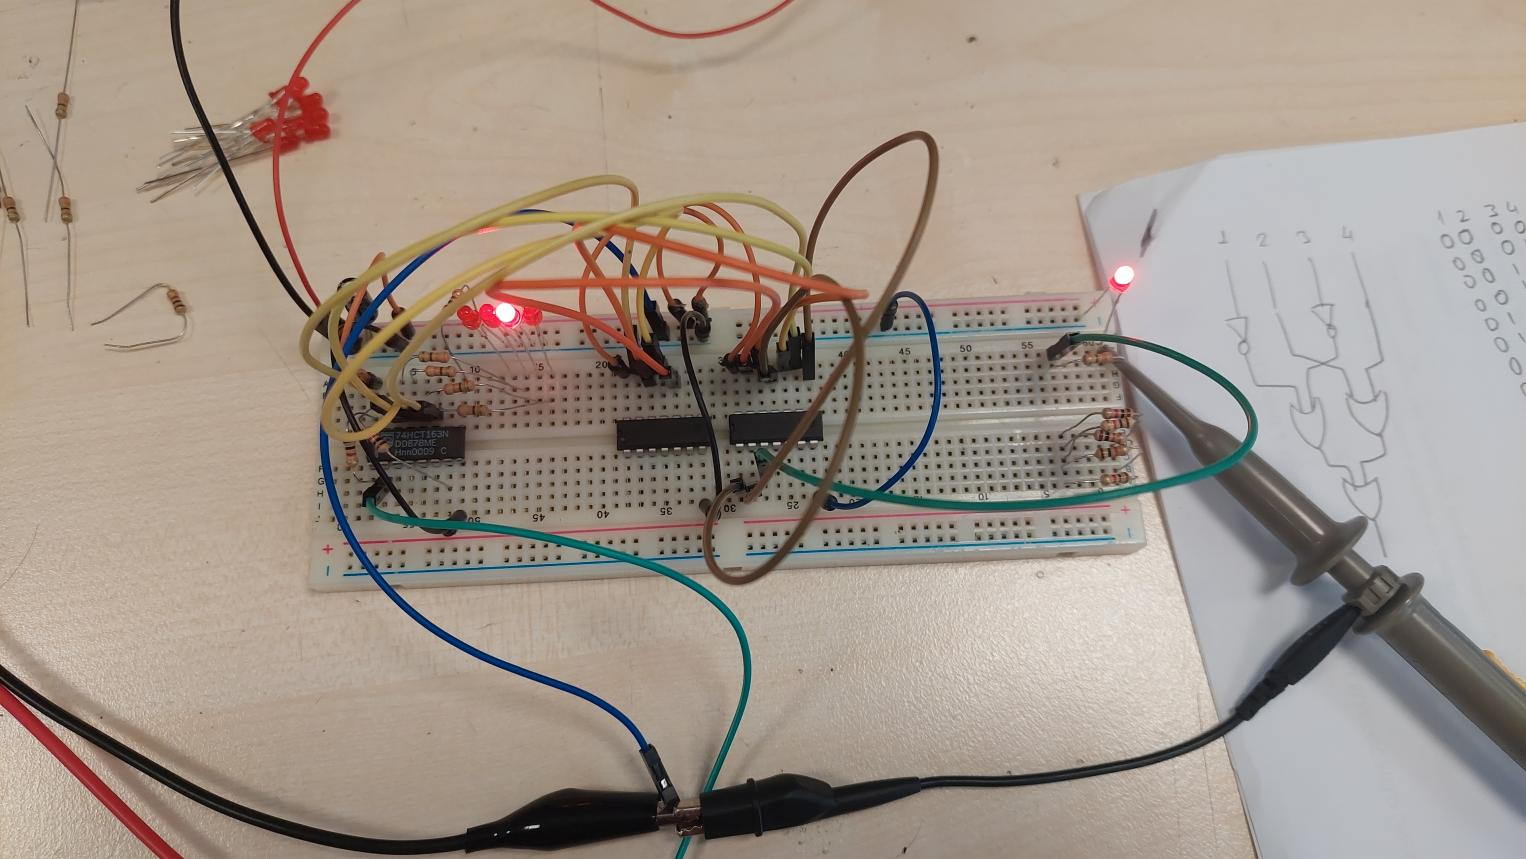
\includegraphics[width=\textwidth]{circuit.jpg}
	\caption{Assembled Circuit}
	\label{fig:circuit}
\end{figure}

\begin{multicols}{2}
\begin{tabular}{cccc|c}
\toprule
D1 & D2 & D3 & D4 & Out\\
\midrule
0 & 0 & 0 & 0 & 1 \\
1 & 0 & 0 & 0 & 1 \\
0 & 1 & 0 & 0 & 1 \\
1 & 1 & 0 & 0 & 1 \\
0 & 0 & 1 & 0 & 1 \\
1 & 0 & 1 & 0 & 0 \\
0 & 1 & 1 & 0 & 1 \\
1 & 1 & 1 & 0 & 1 \\
0 & 0 & 0 & 1 & 1 \\
1 & 0 & 0 & 1 & 1 \\
0 & 1 & 0 & 1 & 1 \\
1 & 1 & 0 & 1 & 1 \\
0 & 0 & 1 & 1 & 1 \\
1 & 0 & 1 & 1 & 1 \\
0 & 1 & 1 & 1 & 1 \\
1 & 1 & 1 & 1 & 1 \\
\bottomrule
\label{table:truth}
\end{tabular}

The circuit on figure \ref{fig:diagram} gives the truth table, shown in the table \ref{table:truth}.
As observed in the circuit on the breadboard and in table \ref{table:truth}, the logic circuit, shown on the figure \ref{fig:diagram}, gives 0 as an output only for the input bits' values 1010.
In order to explain this behavior, the three OR gates can be thought as a single 4-input OR gate, which only output 1 when all of its input are 0's.
This is the case when D1 and D3 are 1 (inverted to 0), and D2 and D4 are 0.
Hence, only when the counting LEDs indicate 1010, the output LED turns off.

\end{multicols}

\begin{wrapfigure}{r}{0.48\textwidth}
	\centering
	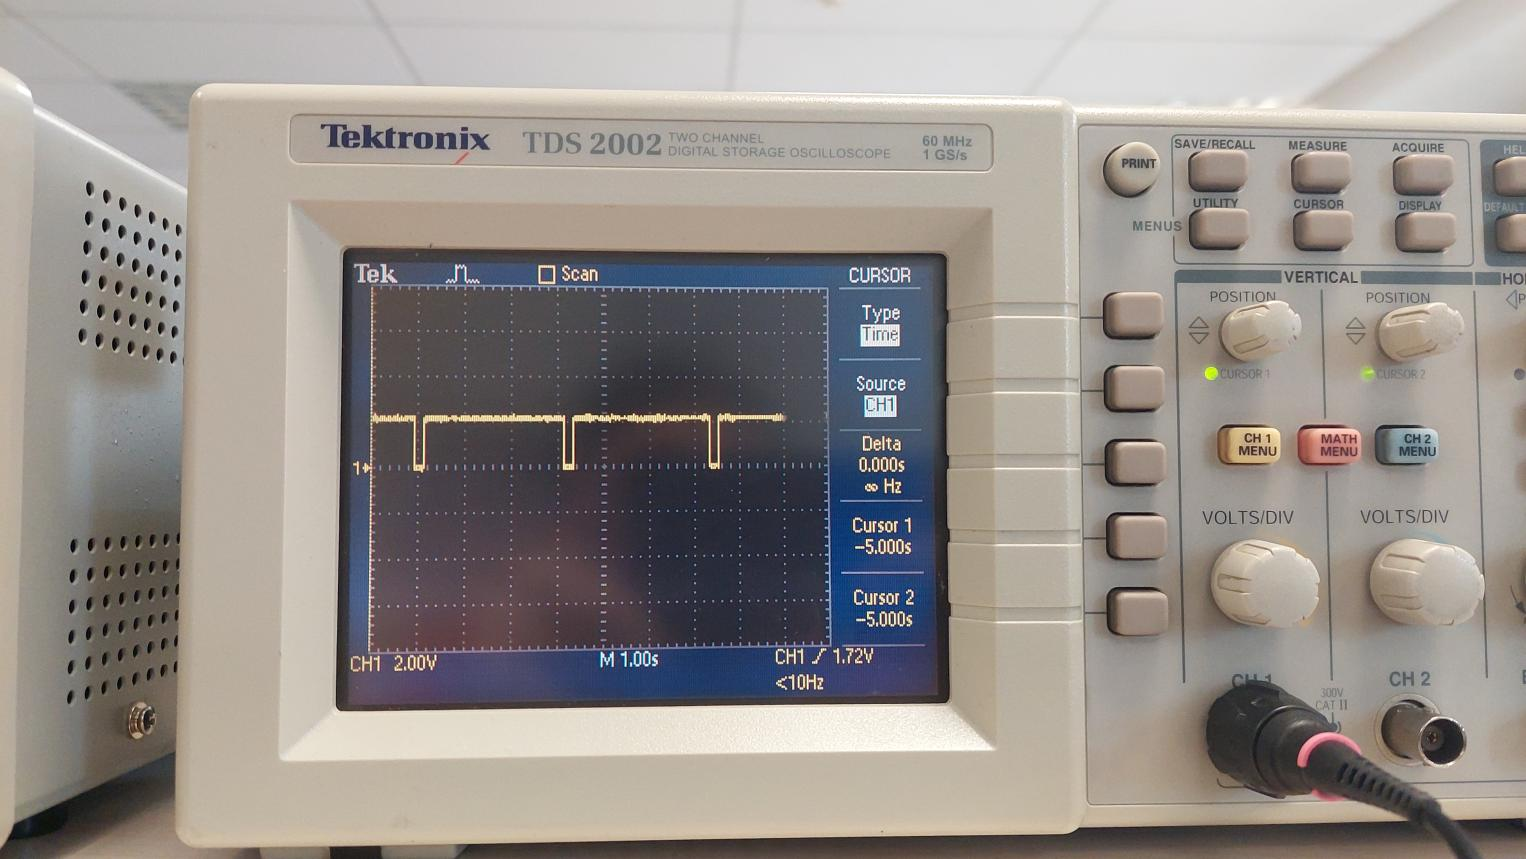
\includegraphics[width=0.48\textwidth]{osc.jpg}
	\caption{Oscilloscope Reading}
	\label{fig:osc}
\end{wrapfigure}

Figure \ref{fig:osc} shows the output of the circuit plotted on an oscilloscope screen.
The plot, as expected, spends 15 seconds in high (5V), and 1 second low logic level ($\sim$ 0V).
Upon careful inspection, it can be seen that the low logic level is not exactly 0V, but around 0.2V.
This is because of the IC's architecture CMOS, and is specified in the datasheet.
According to the 74HC32's datasheet, output voltages up to 0.33V are considered low-level (-40\degree C to +85\degree C).

Although the circuit is run in low speeds (for the LED blinkings to be clearly visible), it is possible to greatly increase the clock speed.
Their datasheets say that 74HC04 and 74HC32 has 18ns propagation delay, and 74HC163 can be used up to 46MHz clock speed.
Hence, the maximum speed for this circuit is the lowest one of $1\over18*10^-9$ Hz or 46MHz, which is 27Mhz (at +25\degree C and 4.5V supply voltage).

\section{Conclusion}

The purpose of this experiment is to practice constructing circuits on a breadboard using logic gate ICs and jumper wires, and visualizing logic levels with LEDs.
This experiment also tested valuable skills an electronics engineer should have, such as fetching information from component datasheets, how to connect components on a breadboard cleanly, and configuring ICs with inputs.

\appendix
\section{Appendix}

\begin{figure}
	\centering
	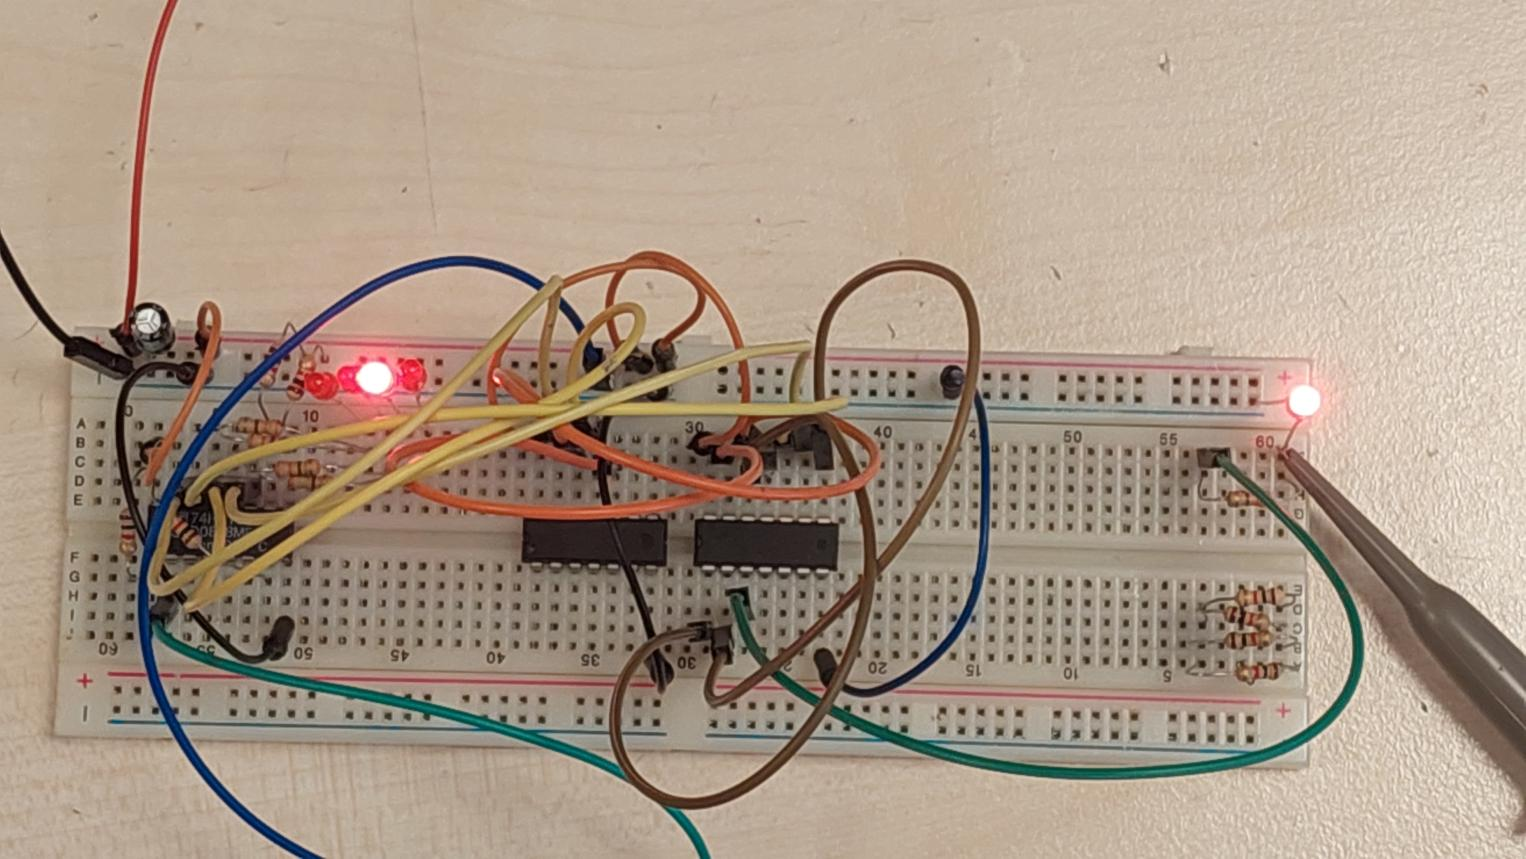
\includegraphics[width=\textwidth]{led-on.jpg}
	\caption{Input 0010}
\end{figure}

\begin{figure}
	\centering
	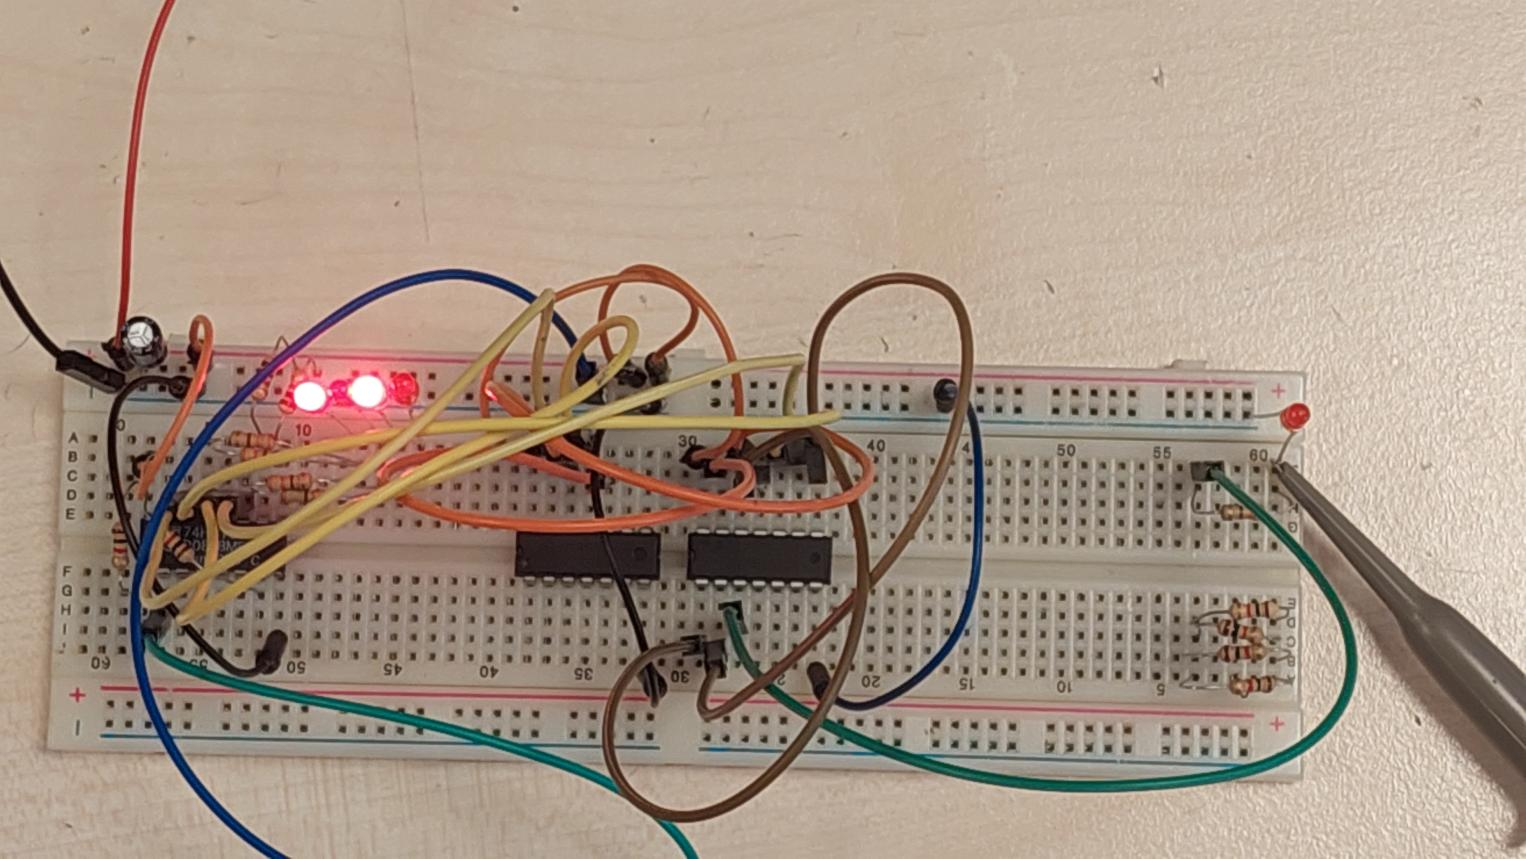
\includegraphics[width=\textwidth]{led-off.jpg}
	\caption{Input 1010}
\end{figure}

\end{document}
